%%%%%%%%%%%%%%%%%%%%%%%%%%%%%%%%%%%%%%%%%%%%%%%%%%%%%%%%%%%%%%%%%%
%%%%%%%%%%%%%%%%%%%%%%%%%%%%%%%%%%%%%%%%%%%%%%%%%%%%%%%%%%%%%%%%%%
%Packages
\documentclass[10pt, a4paper]{article}
\usepackage[top=3cm, bottom=4cm, left=3.5cm, right=3.5cm]{geometry}
\usepackage{amsmath,amsthm,amsfonts,amssymb,amscd, fancyhdr, color, comment, graphicx, environ}
\usepackage{float}
\usepackage{mathrsfs}
\usepackage[math-style=ISO]{unicode-math}
\setmathfont{TeX Gyre Termes Math}
\usepackage{lastpage}
\usepackage[dvipsnames]{xcolor}
\usepackage[framemethod=TikZ]{mdframed}
\usepackage{enumerate}
\usepackage[shortlabels]{enumitem}
\usepackage{fancyhdr}
\usepackage{indentfirst}
\usepackage{listings}
\usepackage{sectsty}
\usepackage{thmtools}
\usepackage{shadethm}
\usepackage{hyperref}
\usepackage{setspace}
\hypersetup{
    colorlinks=true,
    linkcolor=blue,
    filecolor=magenta,      
    urlcolor=blue,
}
\usepackage[utf8]{inputenc}
\usepackage[T1]{fontenc}
\usepackage{hyperref}
\hypersetup{colorlinks=true, linkcolor=blue, filecolor=magenta, urlcolor=cyan,}
\urlstyle{same}
\usepackage{amsmath}
\usepackage{amsfonts}
\usepackage{amssymb}
\usepackage[version=4]{mhchem}
\usepackage{stmaryrd}
\usepackage{graphicx}
\usepackage[export]{adjustbox}
\graphicspath{ {./images/} }
\usepackage{listings}
%%%%%%%%%%%%%%%%%%%%%%%%%%%%%%%%%%%%%%%%%%%%%%%%%%%%%%%%%%%%%%%%%%
%%%%%%%%%%%%%%%%%%%%%%%%%%%%%%%%%%%%%%%%%%%%%%%%%%%%%%%%%%%%%%%%%%
%Environment setup
\mdfsetup{skipabove=\topskip,skipbelow=\topskip}
\newrobustcmd\ExampleText{%
An \textit{inhomogeneous linear} differential equation has the form
\begin{align}
L[v ] = f,
\end{align}
where $L$ is a linear differential operator, $v$ is the dependent
variable, and $f$ is a given non−zero function of the independent
variables alone.
}
\mdfdefinestyle{theoremstyle}{%
linecolor=black,linewidth=1pt,%
frametitlerule=true,%
frametitlebackgroundcolor=gray!20,
innertopmargin=\topskip,
}
\mdtheorem[style=theoremstyle]{Problem}{Problem}
\newenvironment{Solution}{\textbf{Solution.}}

\definecolor{codegreen}{rgb}{0,0.6,0}
\definecolor{codegray}{rgb}{0.5,0.5,0.5}
\definecolor{codepurple}{rgb}{0.58,0,0.82}
\definecolor{backcolour}{rgb}{0.95,0.95,0.92}

\lstdefinestyle{mystyle}{
    backgroundcolor=\color{backcolour},   
    commentstyle=\color{codegreen},
    keywordstyle=\color{magenta},
    numberstyle=\tiny\color{codegray},
    stringstyle=\color{codepurple},
    basicstyle=\ttfamily\footnotesize,
    breakatwhitespace=false,         
    breaklines=true,                 
    captionpos=b,                    
    keepspaces=true,                 
    numbers=left,                    
    numbersep=5pt,                  
    showspaces=false,                
    showstringspaces=false,
    showtabs=false,                  
    tabsize=2
}

\lstset{style=mystyle}
%%%%%%%%%%%%%%%%%%%%%%%%%%%%%%%%%%%%%%%%%%%%%%%%%%%%%%%%%%%%%%%%%%
%%%%%%%%%%%%%%%%%%%%%%%%%%%%%%%%%%%%%%%%%%%%%%%%%%%%%%%%%%%%%%%%%%
%Fill in the appropriate information below
\newcommand{\norm}[1]{\left\lVert#1\right\rVert}     
\newcommand\course{CS5785}                            % <-- course name   
\newcommand\hwnumber{0}                                 % <-- homework number
\newcommand\Information{Arystan Tatishev}                        % <-- personal information
%%%%%%%%%%%%%%%%%%%%%%%%%%%%%%%%%%%%%%%%%%%%%%%%%%%%%%%%%%%%%%%%%%
%%%%%%%%%%%%%%%%%%%%%%%%%%%%%%%%%%%%%%%%%%%%%%%%%%%%%%%%%%%%%%%%%%
%Page setup
\pagestyle{fancy}
\headheight 35pt
\lhead{\today}
\rhead{
\includegraphics[width=2.5cm]{logo-ct.png}}
\lfoot{}
\pagenumbering{arabic}
\cfoot{\small\thepage}
\rfoot{}
\headsep 1.2em
\renewcommand{\baselinestretch}{1.25}
%%%%%%%%%%%%%%%%%%%%%%%%%%%%%%%%%%%%%%%%%%%%%%%%%%%%%%%%%%%%%%%%%%
%%%%%%%%%%%%%%%%%%%%%%%%%%%%%%%%%%%%%%%%%%%%%%%%%%%%%%%%%%%%%%%%%%
%Add new commands here
\renewcommand{\labelenumi}{\alph{enumi})}
\newcommand{\Z}{\mathbb Z}
\newcommand{\R}{\mathbb R}
\newcommand{\Q}{\mathbb Q}
\newcommand{\NN}{\mathbb N}
\newcommand{\PP}{\mathbb P}
\DeclareMathOperator{\Mod}{Mod} 
\renewcommand\lstlistingname{Algorithm}
\renewcommand\lstlistlistingname{Algorithms}
\def\lstlistingautorefname{Alg.}
\newtheorem*{theorem}{Theorem}
\newtheorem*{lemma}{Lemma}
\newtheorem{case}{Case}
\newcommand{\assign}{:=}
\newcommand{\infixiff}{\text{ iff }}
\newcommand{\nobracket}{}
\newcommand{\backassign}{=:}
\newcommand{\tmmathbf}[1]{\ensuremath{\boldsymbol{#1}}}
\newcommand{\tmop}[1]{\ensuremath{\operatorname{#1}}}
\newcommand{\tmtextbf}[1]{\text{{\bfseries{#1}}}}
\newcommand{\tmtextit}[1]{\text{{\itshape{#1}}}}

\newenvironment{itemizedot}{\begin{itemize} \renewcommand{\labelitemi}{$\bullet$}\renewcommand{\labelitemii}{$\bullet$}\renewcommand{\labelitemiii}{$\bullet$}\renewcommand{\labelitemiv}{$\bullet$}}{\end{itemize}}
\catcode`\<=\active \def<{
\fontencoding{T1}\selectfont\symbol{60}\fontencoding{\encodingdefault}}
\catcode`\>=\active \def>{
\fontencoding{T1}\selectfont\symbol{62}\fontencoding{\encodingdefault}}
\catcode`\<=\active \def<{
\fontencoding{T1}\selectfont\symbol{60}\fontencoding{\encodingdefault}}

%%%%%%%%%%%%%%%%%%%%%%%%%%%%%%%%%%%%%%%%%%%%%%%%%%%%%%%%%%%%%%%%%%
%%%%%%%%%%%%%%%%%%%%%%%%%%%%%%%%%%%%%%%%%%%%%%%%%%%%%%%%%%%%%%%%%%
%Begin now!



\begin{document}

\begin{titlepage}
    \begin{center}
        \vspace*{3cm}
            
        \Huge
        \textbf{Assignment}
            
        \vspace{1cm}
        \huge
        Homework\hwnumber
            
        \vspace{1.5cm}
        \Large
            
        \textbf{\Information}                      % <-- author
        
            
        \vfill
        
        A \course \ Homework Assignment
            
        \vspace{1cm}
            
        
\includegraphics[width=0.4\textwidth]{logo-ct.png}
        \\
        
        \Large
        
        \today
            
    \end{center}
\end{titlepage}

%%%%%%%%%%%%%%%%%%%%%%%%%%%%%%%%%%%%%%%%%%%%%%%%%%%%%%%%%%%%%%%%%%
%%%%%%%%%%%%%%%%%%%%%%%%%%%%%%%%%%%%%%%%%%%%%%%%%%%%%%%%%%%%%%%%%%
%Start the assignment now
%%%%%%%%%%%%%%%%%%%%%%%%%%%%%%%%%%%%%%%%%%%%%%%%%%%%%%%%%%%%%%%%%%
%New problem
\newpage

\begin{Problem}
\section{IRIS FLOWERS}
In 1935, Edgar Anderson went to his favourite pasture and recorded the length and width of the sepals and petals on several flowers in the field. For whatever reason, this dataset became one of the oldest and most well-known "sanity-check" datasets around, being cited by countless papers. This class continues this time-honored tradition by using Iris Flowers to sanity-check your Python environment and plotting libraries.

\begin{enumerate}
  \item[1.] Find and download the Iris Flowers dataset from the UC Irvine Machine Learning datasets archive at \href{http://archive.ics.uci.edu/ml/datasets.php}{http://archive.ics.uci.edu/ml/datasets.php} Hint: The iris.names file describes the structure of the dataset. How many features/attributes are there per sample? How many different species are there, and how many samples of each species did Anderson record? 
  \item[2.] Figure out how to parse the dataset you downloaded. Load the samples into an $N \times p$ array, where $N$ is the number of samples and $p$ is the number of attributes per sample. Aditionally, create a $N$-dimensional vector containing each sample's label (species).


Hint: Python has a built-in CSV parser in the csv library, or you can use the "string" .split ( . . ) method.

Hint 2: Here is some code that prints each line in a file:

\begin{lstlisting}[language=Python]
for line in open("/path/to/filename.txt"):
    print "Line contains: "+line
\end{lstlisting}

  \item[3.] To visualize this dataset, we would have to build a $p$-dimensional scatterplot. Unfortunately, we only have $2 \mathrm{D}$ displays so we must reduce the dataset's dimensionality. The easiest way to view the set is to plot two attributes of the data against one another and repeat for each pair of attributes.

Create every possible scatterplot from all pairs of two attributes. (For example, one scatterplot would graph petal length vs sepal width, another would graph petal length vs. sepal length, and so on). Within each scatterplot, the color of each dot should correspond with the sample species. Ideally, we're looking for something like this figure from Wikipedia:

\begin{center}
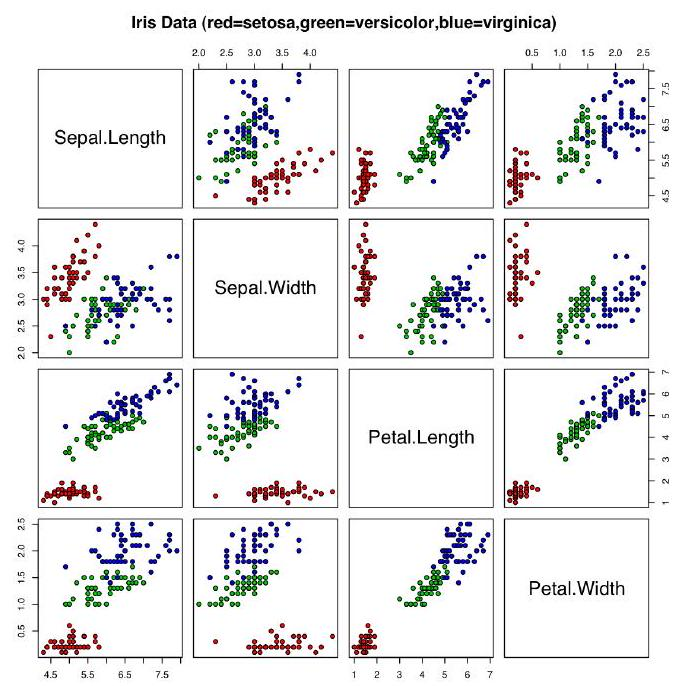
\includegraphics[max width=\textwidth, scale=0.5]{2023_09_05_cccc75871700a893fedfg-3}
\end{center}

But your results do not have to be this ornate. Presenting six separate figures in your report is certainly fine. Be sure to include the source code for all plots!

Hint: This is one way to draw a scatterplot. Use whatever works for you.

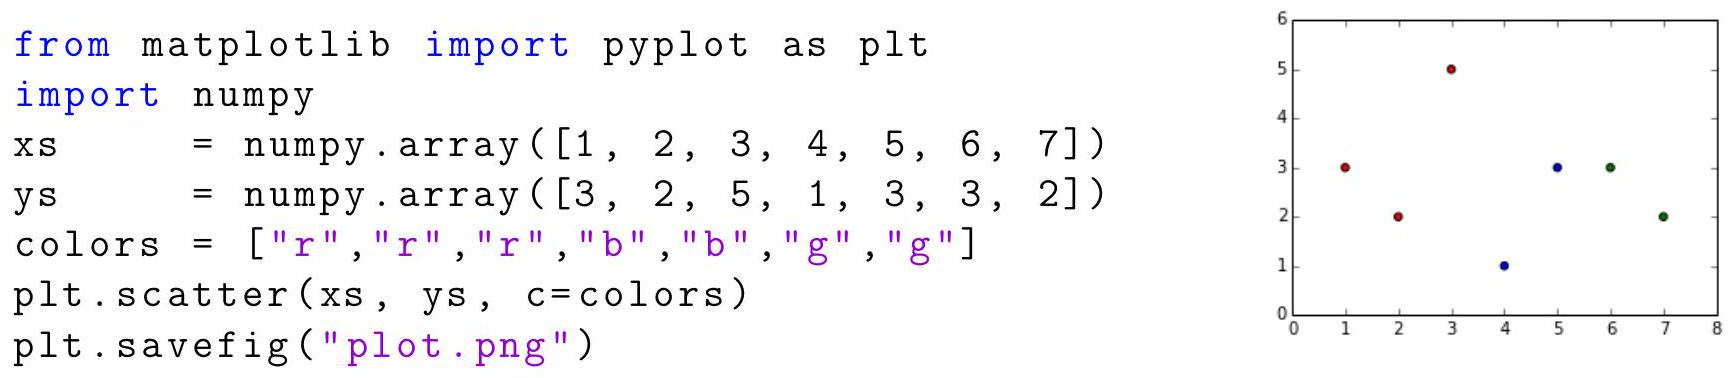
\includegraphics[max width=\textwidth, scale=0.9]{2023_09_05_cccc75871700a893fedfg-3(1)}

Hint: If you would like plots to appear right inside of your Jupyter Notebook, restart the kernel and evaluate the following before running anything else: $\%$ matplotlib inline

Good luck!
\end{enumerate}
\end{Problem}

\begin{Solution}
\begin{enumerate}
    \item[1.] 
    \begin{enumerate}
        \item[Q.] How many features/attributes are there
per sample?
        \item[A.] There are 4 attributes per sample:
        \begin{enumerate}
            \item[1.] sepal length in cm
            \item[2.] sepal width in cm
            \item[3.] petal length in cm
            \item[4.] petal width in cm
        \end{enumerate}
        \item[Q.] How many different species are there, and how many samples of each species did Anderson record?
        \item [A.] There are 3 species, each having 50 samples:
        \begin{enumerate}
            \item[-] Iris Setosa
            \item[-] Iris Versicolour
            \item[-] Iris Virginica
        \end{enumerate}
    \end{enumerate}
    \item[2.] I decided to parse the data by first figuring out how many attributes there are per line. Then I initialized a numpy array with zeros. Every new row in the array is a new sample and each row is a parameter. I also made a numpy array with zeros for every new row samples, so that I can replace each zero with a parameter. Then I add this row to the main dataset array by using vstack. I also stored each samples specie name in a list.
    \begin{lstlisting}[language=Python]
    import numpy as np
    
    with open("./iris/iris.data") as f:
        first_line = f.readline().strip('\n')
        row_length = len(first_line.split(",")) - 1
    raw_data = open("./iris/iris.data")
    full_data = np.zeros((1, row_length))
    sample_labels = []
    for i, line in enumerate(raw_data):
        if i == 150:
            break
        entry_array = np.zeros((1, row_length))
        for idx, parameter in enumerate(line.split(",")):
            if idx == row_length:
                sample_labels.append(parameter.rstrip())
            else:
                entry_array[0, idx] = float(parameter)
        full_data = np.vstack((full_data, entry_array))
    full_data = np.delete(full_data, 0, 0)
    raw_data.close()\end{lstlisting}
    \item[3.] I mimicked the plot that was shown as an example. I created a 4 by 4 subplot grid with the axis names going across the diagonals. I had issues with centering the axis names, because for some reason my axes had different start and end bounds. Then, by going one by one with the subplots, I filled in the data using two for-loops. The output of the graph was identical to the one in the homework problem.
    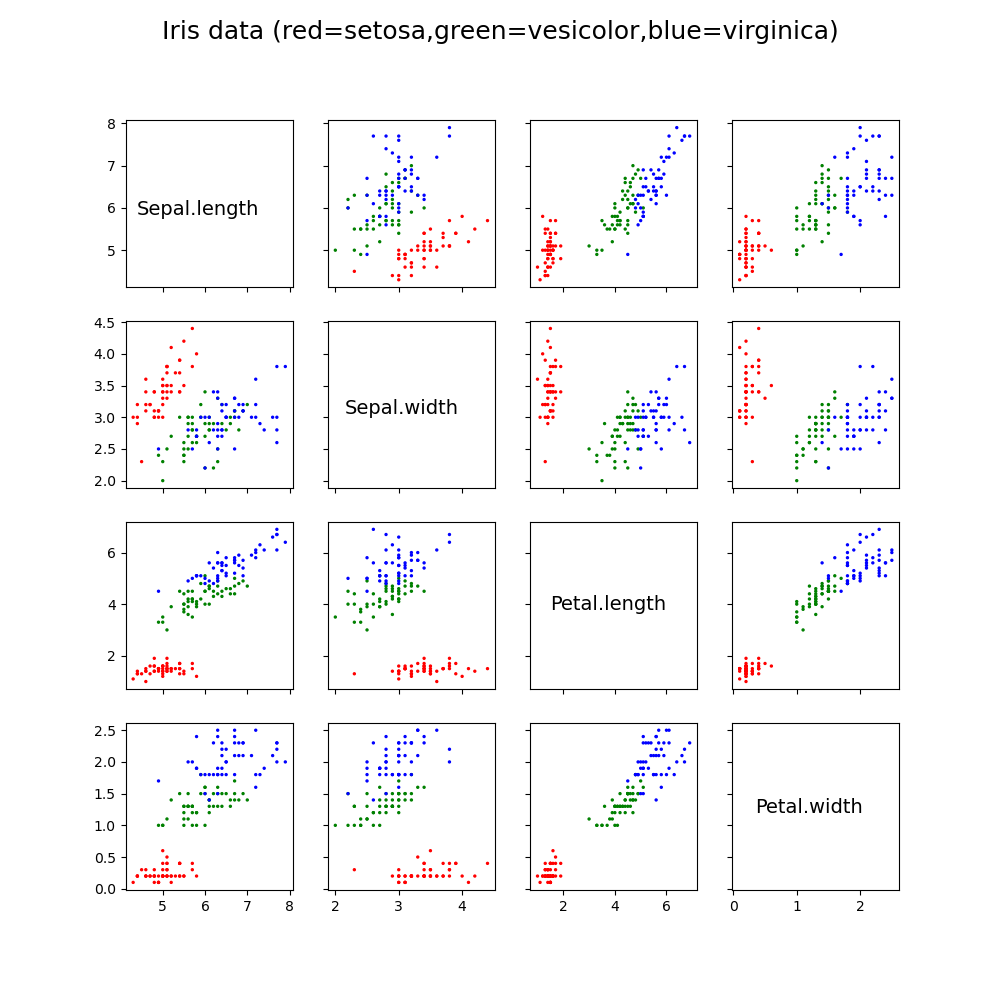
\includegraphics[max width=\textwidth, scale=0.9]{HW0/images/Iris data.png}
    \begin{lstlisting}[language=Python]
from matplotlib import pyplot as plt

colors = []
for label in sample_labels:
    if label == "Iris-setosa":
        colors.append("r")
    elif label == "Iris-versicolor":
        colors.append("g")
    else:
        colors.append("b")

fig, ax = plt.subplots(4, 4, subplot_kw=dict(box_aspect=1), sharex='col', sharey='row', figsize=((10,10)))
fig.suptitle('Iris data (red=setosa,green=vesicolor,blue=virginica)', fontsize=18)
for i in range(4):
    for j in range(4):
        if i == j:
            if i == 0:
                name = "Sepal.length"
            elif i == 1:
                name = "Sepal.width"
            elif i == 2:
                name = "Petal.length"
            else:
                name = "Petal.width"
            ax[i, j].text(full_data[:, j].mean(), full_data[:, j].mean(), name,
                      fontsize=14, ha='center')
        else:
            ax[i, j].scatter(full_data[:, j], full_data[:, i], c = colors, s = 2)
        
plt.savefig ("Iris data.png") \end{lstlisting}
    
\end{enumerate}


\end{Solution}

%%%%%%%%%%%%%%%%%%%%%%%%%%%%%%%%%%%%%%%%%%%%%%%%%%%%%%%%%%%%%%%%%%
%Complete the assignment now
\end{document}

%%%%%%%%%%%%%%%%%%%%%%%%%%%%%%%%%%%%%%%%%%%%%%%%%%%%%%%%%%%%%%%%%%
%%%%%%%%%%%%%%%%%%%%%%%%%%%%%%%%%%%%%%%%%%%%%%%%%%%%%%%%%%%%%%%%%%
